% answers.tex —— 2020 年·天津卷 · 参考答案与详细解析片段
% 由 tools/generate_projects.py 依来源总账自 2020/2020_数学真题_天津_试题.md + 2020/2020_数学真题_天津_解析正文.md + 2020/2020_数学真题_天津_答案要点.md 生成，勿手改（改源 MD 后重跑）


\begin{answer}
\gksolhead{1}{}

\textbf{题目}：

设全集 $U=\{-3,-2,-1,0,1,2,3\}$，集合 $A=\{-1,0,1,2\}$，$B=\{-3,0,2,3\}$，则 $A\cap(\complement_UB)=$\mbox{（　　）}

（A）$\{-3,3\}$；（B）$\{0,2\}$；（C）$\{-1,1\}$；（D）$\{-3,-2,-1,1,3\}$。

\Needspace{4\baselineskip}
\textbf{解析}

\Needspace{5\baselineskip}
先求 $B$ 在 $U$ 中的补集。$U$ 中不属于 $B=\{-3,0,2,3\}$ 的元素是 $-2$，$-1$，$1$，故
\nopagebreak[4]
\[\complement_UB=\{-2,-1,1\}.\]
\Needspace{5\baselineskip}
再与 $A=\{-1,0,1,2\}$ 取交集，只需挑出 $A$ 中属于 $\complement_UB$ 的元素：
\nopagebreak[4]
\[A\cap(\complement_UB)=\{-1,1\}.\]

选 C。

\gkanswer{答案：C。$\complement_UB=\{-2,-1,1\}$，与 $A=\{-1,0,1,2\}$ 取交集得 $\{-1,1\}$。}

\end{answer}
\begin{answer}
\gksolhead{2}{}

\textbf{题目}：

设 $a\in\mathbf R$，则「$a>1$」是「$a^2>a$」的\mbox{（　　）}

（A）充分不必要条件；（B）必要不充分条件；（C）充要条件；（D）既不充分也不必要条件。

\Needspace{4\baselineskip}
\textbf{解析}

\Needspace{5\baselineskip}
先看充分性。若 $a>1$，则 $a>0$ 且 $a-1>0$，于是
\nopagebreak[4]
\[a^2-a=a(a-1)>0,\]
即 $a^2>a$ 成立。故「$a>1$」是「$a^2>a$」的充分条件。

\Needspace{5\baselineskip}
再看必要性。$a^2>a$ 即 $a(a-1)>0$，解得
\nopagebreak[4]
\[a<0\quad\text{\text{或}}\quad a>1 .\]
取 $a=-1$，此时 $a^2=1>-1=a$，条件「$a^2>a$」成立，但「$a>1$」不成立。故「$a>1$」不是「$a^2>a$」的必要条件。

综上，「$a>1$」是「$a^2>a$」的充分不必要条件。

选 A。

\gkanswer{答案：A。$a>1$ 时 $a^2-a=a(a-1)>0$，反之 $a^2>a$ 的解为 $a<0$ 或 $a>1$，故为充分不必要条件。}

\end{answer}
\begin{answer}
\gksolhead{3}{}

\textbf{题目}：

函数 $y=\dfrac{4x}{x^2+1}$ 的图象大致为\mbox{（　　）}
\nopagebreak[4]
\begin{center}% 2020 天津卷 第 3 题：函数 y = 4x/(x^2+1) 的四个图象选项（2×2 四联图）
% 来源 PDF：普通高考/2020/2020天津.pdf 第 1 页（A3 横排），印面 1131，第 3 题题干下方
% 逐格核对原页矢量曲线（600 dpi 渲染并读 SVG 路径，单位 pt）后确认四幅互不相同：
%   (A) 奇函数；x 轴刻度 1 处取最大值 2（曲线最高点横坐标与刻度 1 重合），
%       x=-1 处取最小值 -2，两端趋于 0 —— 即 y=4x/(x^2+1)；
%   (B) 与 (A) 关于 x 轴对称，最大值在 x=-1，最小值在 x=1 —— 即 y=-4x/(x^2+1)；
%   (C) 偶函数；x=±1 处各取最大值 2，原点处为尖点且函数值为 0 —— 即 y=4|x|/(x^2+1)；
%   (D) 与 (C) 关于 x 轴对称，x=±1 处各取最小值 -2 —— 即 y=-4|x|/(x^2+1)。
% 原页每幅图均画：x 轴（右端箭头、标 x）、y 轴（上端箭头、标 y）、原点 O、
%   x 轴刻度 1、y 轴刻度 2；坐标轴在 x 方向总长约 13.6 个单位，曲线自 -6.5 画到 6.5。
\begin{tikzpicture}[font=\small,>=Stealth,line cap=round,line join=round]
  % (A) 左上：y = 4x/(x^2+1)
  \begin{scope}[shift={(0,3.05)},x=0.32cm,y=0.42cm]
    \draw[->] (-6.9,0)--(7.0,0) node[below,inner sep=2pt] {$x$};
    \draw[->] (0,-2.5)--(0,3.05) node[left,inner sep=2pt] {$y$};
    \node[below left,inner sep=1pt] at (0,0) {$O$};
    \draw (1,0.12)--(1,-0.12) node[below,inner sep=6pt] {$1$};
    \draw (0.24,2)--(-0.30,2);
    \node[above left,inner sep=2pt] at (-0.32,2) {$2$};
    \draw[line width=0.9pt,domain=-6.5:6.5,samples=300,smooth]
      plot (\x,{4*\x/(\x*\x+1)});
    \node at (-5.6,-3.35) {(A)};
  \end{scope}
  % (B) 右上：y = -4x/(x^2+1)
  \begin{scope}[shift={(4.65,3.05)},x=0.32cm,y=0.42cm]
    \draw[->] (-6.9,0)--(7.0,0) node[below,inner sep=2pt] {$x$};
    \draw[->] (0,-2.5)--(0,3.05) node[left,inner sep=2pt] {$y$};
    \node[below left,inner sep=1pt] at (0,0) {$O$};
    \draw (1,0.12)--(1,-0.12) node[below,inner sep=6pt] {$1$};
    \draw (0.24,2)--(-0.30,2);
    \node[above left,inner sep=2pt] at (-0.32,2) {$2$};
    \draw[line width=0.9pt,domain=-6.5:6.5,samples=300,smooth]
      plot (\x,{-4*\x/(\x*\x+1)});
    \node at (-5.6,-3.35) {(B)};
  \end{scope}
  % (C) 左下：y = 4|x|/(x^2+1)
  \begin{scope}[shift={(0,0.30)},x=0.32cm,y=0.42cm]
    \draw[->] (-6.9,0)--(7.0,0) node[below,inner sep=2pt] {$x$};
    \draw[->] (0,-2.5)--(0,3.05) node[left,inner sep=2pt] {$y$};
    \node[below left,inner sep=1pt] at (0,0) {$O$};
    \draw (1,0.12)--(1,-0.12) node[below,inner sep=6pt] {$1$};
    \draw (0.24,2)--(-0.30,2);
    \node[above left,inner sep=2pt] at (-0.32,2) {$2$};
    \draw[line width=0.9pt,domain=-6.5:0,samples=160,smooth]
      plot (\x,{4*abs(\x)/(\x*\x+1)});
    \draw[line width=0.9pt,domain=0:6.5,samples=160,smooth]
      plot (\x,{4*abs(\x)/(\x*\x+1)});
    \node at (-5.6,-3.35) {(C)};
  \end{scope}
  % (D) 右下：y = -4|x|/(x^2+1)
  \begin{scope}[shift={(4.65,0.30)},x=0.32cm,y=0.42cm]
    \draw[->] (-6.9,0)--(7.0,0) node[below,inner sep=2pt] {$x$};
    \draw[->] (0,-2.5)--(0,3.05) node[left,inner sep=2pt] {$y$};
    \node[below left,inner sep=1pt] at (0,0) {$O$};
    \draw (1,0.12)--(1,-0.12) node[below,inner sep=6pt] {$1$};
    \draw (0.24,2)--(-0.30,2);
    \node[above left,inner sep=2pt] at (-0.32,2) {$2$};
    \draw[line width=0.9pt,domain=-6.5:0,samples=160,smooth]
      plot (\x,{-4*abs(\x)/(\x*\x+1)});
    \draw[line width=0.9pt,domain=0:6.5,samples=160,smooth]
      plot (\x,{-4*abs(\x)/(\x*\x+1)});
    \node at (-5.6,-3.35) {(D)};
  \end{scope}
\end{tikzpicture}
\end{center}
\nopagebreak[4]
\Needspace{4\baselineskip}
\textbf{解析}

\Needspace{5\baselineskip}
记 $f(x)=\dfrac{4x}{x^2+1}$，其定义域为 $\mathbf R$，且
\nopagebreak[4]
\[f(-x)=\frac{-4x}{x^2+1}=-f(x),\]
故 $f$ 为奇函数，图象关于原点对称；又 $x>0$ 时 $f(x)>0$，$x<0$ 时 $f(x)<0$，且 $x\to\pm\infty$ 时 $f(x)\to0$。

\Needspace{5\baselineskip}
求导：
\nopagebreak[4]
\[f'(x)=\frac{4(x^2+1)-4x\cdot2x}{(x^2+1)^2}=\frac{4(1-x^2)}{(x^2+1)^2}.\]
\Needspace{5\baselineskip}
故 $f$ 在 $(-\infty,-1)$ 上递减，在 $(-1,1)$ 上递增，在 $(1,+\infty)$ 上递减，极大值
\nopagebreak[4]
\[f(1)=\frac42=2,\]
\Needspace{5\baselineskip}
极小值
\nopagebreak[4]
\[f(-1)=-2 .\]

逐格对照原页四幅图：

\begin{itemize}
\item （A）奇函数，$x>0$ 时图象先升后降、最高点恰在 $x$ 轴刻度 $1$ 的正上方且高度为 $2$，$x<0$ 时最低点为 $-2$，两端趋于 $0$——与上述特征完全一致；
\item （B）与（A）关于 $x$ 轴对称，最大值出现在 $x=-1$，是 $y=-\dfrac{4x}{x^2+1}$ 的图象；
\item （C）为偶函数，$x=\pm1$ 处各有一个高度 $2$ 的极大值，原点处是函数值为 $0$ 的尖点，对应 $y=\dfrac{4|x|}{x^2+1}$；
\item （D）与（C）关于 $x$ 轴对称，$x=\pm1$ 处各有一个极小值 $-2$，对应 $y=-\dfrac{4|x|}{x^2+1}$。
\end{itemize}

四幅图互不相同，只有（A）符合 $y=\dfrac{4x}{x^2+1}$。

选 A。

\gkanswer{答案：A。$y=\dfrac{4x}{x^2+1}$ 是奇函数，$x>0$ 时在 $x=1$ 处取最大值 $2$，两端趋于 $0$，与（A）一致。}

\end{answer}
\begin{answer}
\gksolhead{4}{}

\textbf{题目}：

从一批零件中抽取 $80$ 个，测量其直径（单位：mm），将所得数据分为 $9$ 组：$[5.31,5.33)$，$[5.33,5.35)$，$\cdots$，$[5.45,5.47)$，$[5.47,5.49]$，并整理得到如下频率分布直方图，则在被抽取的零件中，直径落在区间 $[5.43,5.47)$ 内的个数为\mbox{（　　）}
\nopagebreak[4]
\begin{center}% 2020 天津卷 第 4 题：频率分布直方图
% 来源 PDF：普通高考/2020/2020天津.pdf 第 1 页（A3 横排），印面 1131，第 4 题题干下方
% 几何按原页矢量数据换算：9 个等宽组 [5.31,5.33) … [5.47,5.49]，
%   矩形高度（频率/组距）依次为 1.25、3.75、2.50、7.50、10.00、8.75、6.25、5.00、5.00，
%   组距 0.02，故各矩形面积（频率）依次为 0.025、0.075、0.05、0.15、0.20、0.175、0.125、0.10、0.10，
%   合计 1.00，与 80 个样本一致。
% 纵轴虚线只标 1.25 的整数倍刻度，自 1.25 起至 10.00（原页即 8 条虚线）；
% 横轴自 5.31 起每 0.02 标一组端点，末尾 5.49；原点左侧有断裂符号，0 标在断裂符号之外。
\begin{tikzpicture}[font=\small,
  x=0.60cm, y=0.26cm, line cap=round, line join=round]
  % 坐标轴（左端留出断裂符号与 0 的位置）
  \draw[->] (-1.35,0)--(10.35,0) node[right,inner sep=4pt] {直径/mm};
  \draw[->] (0,0)--(0,11.6) node[above,inner sep=4pt] {$\dfrac{\text{频率}}{\text{组距}}$};
  % 断裂符号
  \draw (-0.78,0.10)--(-0.36,-0.34) (-0.78,-0.34)--(-0.36,0.10);
  \node[below,inner sep=4pt] at (-1.18,0) {$0$};
  % 纵向虚线刻度 1.25—10.00
  \foreach \h/\lab in {1.25/1.25,2.50/2.50,3.75/3.75,5.00/5.00,
                       6.25/6.25,7.50/7.50,8.75/8.75,10.00/10.00}{
    \draw[dashed,line width=0.4pt] (0,\h)--(9,\h);
    \draw (-0.14,\h)--(0,\h);
    \node[left,inner sep=2pt,font=\scriptsize] at (-0.12,\h) {\lab};
  }
  % 9 个矩形
  \foreach \i/\h in {0/1.25,1/3.75,2/2.50,3/7.50,4/10.00,5/8.75,6/6.25,7/5.00,8/5.00}{
    \draw[line width=0.6pt] (\i,0) rectangle (\i+1,\h);
  }
  % 横轴刻度与标签
  \foreach \i/\lab in {0/5.31,1/5.33,2/5.35,3/5.37,4/5.39,5/5.41,
                       6/5.43,7/5.45,8/5.47,9/5.49}{
    \draw (\i,0)--(\i,-0.28);
    \node[below,inner sep=2pt,font=\scriptsize] at (\i,0) {\lab};
  }
\end{tikzpicture}
\end{center}
\nopagebreak[4]
（A）$10$；（B）$18$；（C）$20$；（D）$36$。

\Needspace{4\baselineskip}
\textbf{解析}

\Needspace{5\baselineskip}
纵轴是「频率／组距」，组距为
\nopagebreak[4]
\[5.33-5.31=0.02,\]
\Needspace{5\baselineskip}
故每个矩形的面积等于该组的频率。由直方图读得 $9$ 个矩形的高度依次为
\nopagebreak[4]
\[1.25,\ 3.75,\ 2.50,\ 7.50,\ 10.00,\ 8.75,\ 6.25,\ 5.00,\ 5.00 .\]
\Needspace{5\baselineskip}
先验证数据自洽：高度之和为
\nopagebreak[4]
\[1.25+3.75+2.50+7.50+10.00+8.75+6.25+5.00+5.00=50,\]
乘以组距 $0.02$ 得总频率 $1.00$，与频率和为 $1$ 相符。

\Needspace{5\baselineskip}
区间 $[5.43,5.47)$ 恰好覆盖两组：
\nopagebreak[4]
\[[5.43,5.45)\ \text{\text{与}}\ [5.45,5.47),\]
\Needspace{5\baselineskip}
其高度分别为 $6.25$ 与 $5.00$，故该区间的频率为
\nopagebreak[4]
\[(6.25+5.00)\times0.02=11.25\times0.02=0.225 .\]
\Needspace{5\baselineskip}
样本容量为 $80$，所求个数为
\nopagebreak[4]
\[80\times0.225=18 .\]

选 B。

\gkanswer{答案：B。区间 $[5.43,5.47)$ 含两组，频率为 $(6.25+5.00)\times0.02=0.225$，个数为 $80\times0.225=18$。}

\end{answer}
\begin{answer}
\gksolhead{5}{}

\textbf{题目}：

若棱长为 $2\sqrt3$ 的正方体的顶点都在同一球面上，则该球的表面积为\mbox{（　　）}

（A）$12\pi$；（B）$24\pi$；（C）$36\pi$；（D）$144\pi$。

\Needspace{4\baselineskip}
\textbf{解析}

正方体的八个顶点都在球面上，故球是正方体的外接球，球的直径等于正方体的体对角线长。

\Needspace{5\baselineskip}
棱长 $a=2\sqrt3$，体对角线长为
\nopagebreak[4]
\[\sqrt{a^2+a^2+a^2}=\sqrt3\,a=\sqrt3\times2\sqrt3=6 .\]
\Needspace{5\baselineskip}
故 $2R=6$，即 $R=3$。球的表面积为
\nopagebreak[4]
\[S=4\pi R^2=4\pi\times9=36\pi .\]

选 C。

\gkanswer{答案：C。正方体体对角线为球的直径，$2R=2\sqrt3\times\sqrt3=6$，$R=3$，表面积 $4\pi R^2=36\pi$。}

\end{answer}
\begin{answer}
\gksolhead{6}{}

\textbf{题目}：

设 $a=3^{0.7}$，$b=\left(\dfrac13\right)^{-0.8}$，$c=\log_{0.7}0.8$，则 $a$，$b$，$c$ 的大小关系为\mbox{（　　）}

（A）$a<b<c$；（B）$b<a<c$；（C）$b<c<a$；（D）$c<a<b$。

\Needspace{4\baselineskip}
\textbf{解析}

三个数分别化简：

\Needspace{5\baselineskip}
（1）$a=3^{0.7}$，底数 $3>1$，指数 $0.7\in(0,1)$，故
\nopagebreak[4]
\[1<a=3^{0.7}<3^1=3 .\]

\Needspace{5\baselineskip}
（2）$b=\left(\dfrac13\right)^{-0.8}=3^{0.8}$，同样底数大于 $1$，由 $0.8>0.7$ 得
\nopagebreak[4]
\[b=3^{0.8}>3^{0.7}=a .\]

\Needspace{5\baselineskip}
（3）$c=\log_{0.7}0.8$。底数 $0.7\in(0,1)$，故 $y=\log_{0.7}x$ 在 $(0,+\infty)$ 上递减。由
\nopagebreak[4]
\[0.7^0=1>0.8>0.7=0.7^1\]
\Needspace{5\baselineskip}
两边取 $\log_{0.7}$（递减，不等号反向）得
\nopagebreak[4]
\[0=\log_{0.7}1<c=\log_{0.7}0.8<\log_{0.7}0.7=1 .\]

\Needspace{5\baselineskip}
于是
\nopagebreak[4]
\[c<1<a<b,\qquad\text{\text{即}}\quad c<a<b .\]
数值复核：$a\approx2.158$，$b\approx2.408$，$c\approx0.626$，与上式一致。

选 D。

\gkanswer{答案：D。$a=3^{0.7}\approx2.158$，$b=3^{0.8}\approx2.408$，$c=\log_{0.7}0.8\approx0.626$，故 $c<a<b$。}

\end{answer}
\begin{answer}
\gksolhead{7}{}

\textbf{题目}：

设双曲线 $C$ 的方程为 $\dfrac{x^2}{a^2}-\dfrac{y^2}{b^2}=1$（$a>0$，$b>0$），过抛物线 $y^2=4x$ 的焦点和点 $(0,b)$ 的直线为 $l$。若 $C$ 的一条渐近线与 $l$ 平行，另一条渐近线与 $l$ 垂直，则双曲线 $C$ 的方程为\mbox{（　　）}

（A）$\dfrac{x^2}{4}-\dfrac{y^2}{4}=1$；（B）$x^2-\dfrac{y^2}{4}=1$；（C）$\dfrac{x^2}{4}-y^2=1$；（D）$x^2-y^2=1$。

\Needspace{4\baselineskip}
\textbf{解析}

\Needspace{5\baselineskip}
抛物线 $y^2=4x$ 的焦点为 $F(1,0)$。直线 $l$ 过 $F(1,0)$ 与 $(0,b)$，其斜率为
\nopagebreak[4]
\[k_l=\frac{b-0}{0-1}=-b .\]

双曲线 $\dfrac{x^2}{a^2}-\dfrac{y^2}{b^2}=1$ 的两条渐近线为 $y=\pm\dfrac bax$，斜率分别为 $\dfrac ba$ 与 $-\dfrac ba$。

\Needspace{5\baselineskip}
由题意，一条渐近线与 $l$ 平行，另一条与 $l$ 垂直。取与 $l$ 平行的那条斜率为 $-\dfrac ba$，则
\nopagebreak[4]
\[-\frac ba=-b\ \Longrightarrow\ a=1 .\]
\Needspace{5\baselineskip}
另一条渐近线斜率为 $\dfrac ba=b$，与 $l$ 垂直给出
\nopagebreak[4]
\[b\cdot(-b)=-1\ \Longrightarrow\ b^2=1\ \Longrightarrow\ b=1\ (\text{\text{因}}\ b>0).\]
\Needspace{5\baselineskip}
故 $a=b=1$，双曲线方程为
\nopagebreak[4]
\[x^2-y^2=1 .\]

选 D。

\gkanswer{答案：D。抛物线焦点为 $(1,0)$，$l$ 的斜率为 $-b$；渐近线斜率为 $\pm\dfrac ba$，由平行得 $a=1$，由垂直得 $b^2=a=1$，故 $C:x^2-y^2=1$。}

\end{answer}
\begin{answer}
\gksolhead{8}{}

\textbf{题目}：

已知函数 $f(x)=\sin\left(x+\dfrac\pi3\right)$。给出下列结论：

① $f(x)$ 的最小正周期为 $2\pi$；

② $f\left(\dfrac\pi2\right)$ 是 $f(x)$ 的最大值；

③ 把函数 $y=\sin x$ 的图象上所有点向左平移 $\dfrac\pi3$ 个单位长度，可得到函数 $y=f(x)$ 的图象。

其中所有正确结论的序号是\mbox{（　　）}

（A）①；（B）①③；（C）②③；（D）①②③。

\Needspace{4\baselineskip}
\textbf{解析}

逐条判断。

① $f(x)=\sin\left(x+\dfrac\pi3\right)$ 由 $\sin x$ 平移得到，最小正周期仍为 $2\pi$。① 正确。

\Needspace{5\baselineskip}
② 计算
\nopagebreak[4]
\[f\left(\frac\pi2\right)=\sin\left(\frac\pi2+\frac\pi3\right)=\sin\frac{5\pi}6=\frac12 .\]
而 $f(x)$ 的最大值为 $1$（在 $x+\dfrac\pi3=\dfrac\pi2+2k\pi$ 即 $x=\dfrac\pi6+2k\pi$ 处取到），故 $f\left(\dfrac\pi2\right)$ 不是最大值。② 错误。

\Needspace{5\baselineskip}
③ 把 $y=\sin x$ 图象上所有点向左平移 $\dfrac\pi3$ 个单位，所得图象对应的函数为
\nopagebreak[4]
\[y=\sin\left(x+\frac\pi3\right)=f(x).\]
③ 正确。

故正确结论为 ①③。

选 B。

\gkanswer{答案：B。最小正周期为 $2\pi$（①真）；$f\left(\dfrac\pi2\right)=\sin\dfrac{5\pi}6=\dfrac12$ 不是最大值（②假）；左移 $\dfrac\pi3$ 即得 $f(x)$（③真）。}

\end{answer}
\begin{answer}
\gksolhead{9}{}

\textbf{题目}：

已知函数 $f(x)=\begin{cases}x^3,&x\geqslant0,\\-x,&x<0.\end{cases}$ 若函数 $g(x)=f(x)-|kx^2-2x|$（$k\in\mathbf R$）恰有 $4$ 个零点，则 $k$ 的取值范围是\mbox{（　　）}

（A）$\left(-\infty,-\dfrac12\right)\cup\left(2\sqrt2,+\infty\right)$；（B）$\left(-\infty,-\dfrac12\right)\cup\left(0,2\sqrt2\right)$；（C）$(-\infty,0)\cup\left(0,2\sqrt2\right)$；（D）$(-\infty,0)\cup\left(2\sqrt2,+\infty\right)$。

\Needspace{4\baselineskip}
\textbf{解析}

先注意 $x=0$ 处：$f(0)=0$，$|k\cdot0^2-2\cdot0|=0$，故 $g(0)=0$ 恒成立，$x=0$ 是 $g$ 的一个零点（与 $k$ 无关）。

\Needspace{5\baselineskip}
以下讨论 $x\neq0$。此时 $|kx^2-2x|=|x|\cdot|kx-2|$，方程 $g(x)=0$ 即
\nopagebreak[4]
\[f(x)=|x|\,|kx-2| .\]

\Needspace{5\baselineskip}
\textbf{（i）$x>0$。} $f(x)=x^3$，$|x|=x$，方程化为
\nopagebreak[4]
\[x^3=x|kx-2|\ \Longrightarrow\ x^2=|kx-2|,\]
\Needspace{5\baselineskip}
即
\nopagebreak[4]
\[kx-2=x^2\quad\text{\text{或}}\quad kx-2=-x^2,\]
\Needspace{5\baselineskip}
解得
\nopagebreak[4]
\[k=x+\frac2x\quad\text{\text{或}}\quad k=\frac2x-x .\]

记 $h_1(x)=x+\dfrac2x$（$x>0$），由均值不等式 $h_1(x)\geqslant2\sqrt2$，等号在 $x=\sqrt2$ 处成立；且 $h_1$ 在 $(0,\sqrt2)$ 上递减、在 $(\sqrt2,+\infty)$ 上递增，值域为 $[2\sqrt2,+\infty)$。故方程 $h_1(x)=k$ 在 $x>0$ 上：$k>2\sqrt2$ 时有 $2$ 个解，$k=2\sqrt2$ 时有 $1$ 个解，$k<2\sqrt2$ 时无解。

记 $h_2(x)=\dfrac2x-x$（$x>0$），它在 $(0,+\infty)$ 上严格递减，值域为 $\mathbf R$，故 $h_2(x)=k$ 对任意实数 $k$ 恰有 $1$ 个正解。

\Needspace{5\baselineskip}
于是 $x>0$ 时 $g$ 的零点个数为
\nopagebreak[4]
\[\begin{cases}3,&k>2\sqrt2,\\ 2,&k=2\sqrt2,\\ 1,&k<2\sqrt2.\end{cases}\]

\Needspace{5\baselineskip}
\textbf{（ii）$x<0$。} $f(x)=-x$，$|x|=-x$，方程化为
\nopagebreak[4]
\[-x=(-x)|kx-2|\ \Longrightarrow\ |kx-2|=1,\]
\Needspace{5\baselineskip}
即
\nopagebreak[4]
\[kx-2=1\quad\text{\text{或}}\quad kx-2=-1,\]
\Needspace{5\baselineskip}
解得
\nopagebreak[4]
\[x=\frac3k\quad\text{\text{或}}\quad x=\frac1k .\]
\Needspace{5\baselineskip}
这两解都为负数当且仅当 $k<0$；$k>0$ 时两解为正，与 $x<0$ 矛盾，应舍去；$k=0$ 时方程 $|{-2}|=1$ 不成立，无解。故 $x<0$ 时零点个数为
\nopagebreak[4]
\[\begin{cases}2,&k<0,\\ 0,&k\geqslant0.\end{cases}\]

\textbf{（iii）合并。} 零点总数为

\begin{center}
\begin{tabular}{ccccc}
\toprule
$k$ 的范围 & $x<0$ & $x=0$ & $x>0$ & 合计 \\
\midrule
$k<0$ & $2$ & $1$ & $1$ & $4$ \\
$k=0$ & $0$ & $1$ & $1$ & $2$ \\
$0<k<2\sqrt2$ & $0$ & $1$ & $1$ & $2$ \\
$k=2\sqrt2$ & $0$ & $1$ & $2$ & $3$ \\
$k>2\sqrt2$ & $0$ & $1$ & $3$ & $4$ \\
\bottomrule
\end{tabular}
\end{center}

\Needspace{5\baselineskip}
恰有 $4$ 个零点当且仅当 $k<0$ 或 $k>2\sqrt2$，即
\nopagebreak[4]
\[k\in(-\infty,0)\cup(2\sqrt2,+\infty).\]

数值复核：$k=-1$ 时零点为 $-3$，$-1$，$0$，$2$，共 $4$ 个；$k=3$ 时零点为 $0$，$0.5616$，$1$，$2$，共 $4$ 个；$k=2$ 时零点为 $0$，$0.7321$，共 $2$ 个；$k=2\sqrt2$ 时零点为 $0$，$0.5858$，$\sqrt2$，共 $3$ 个；$k=0$ 时零点为 $0$，$\sqrt2$，共 $2$ 个。与上表一致。

选 D。

\gkanswer{答案：D。$x\geqslant0$ 时零点满足 $k=x+\dfrac2x$ 或 $k=\dfrac2x-x$，$x<0$ 时零点为 $\dfrac1k$、$\dfrac3k$（需 $k<0$）；$x=0$ 恒为零点。故 $k<0$ 给 $4$ 个零点、$0\leqslant k\leqslant2\sqrt2$ 给 $2$ 或 $3$ 个、$k>2\sqrt2$ 给 $4$ 个，即 $k\in(-\infty,0)\cup(2\sqrt2,+\infty)$。}

\end{answer}
\begin{answer}
\gksolhead{10}{}

\textbf{题目}：

$\mathrm i$ 是虚数单位，复数 $\dfrac{8-\mathrm i}{2+\mathrm i}=$\gkblank{}。

\Needspace{4\baselineskip}
\textbf{解析}

\Needspace{5\baselineskip}
对分母实数化，分子分母同乘 $2-\mathrm i$：
\nopagebreak[4]
\[\frac{8-\mathrm i}{2+\mathrm i}=\frac{(8-\mathrm i)(2-\mathrm i)}{(2+\mathrm i)(2-\mathrm i)}=\frac{16-8\mathrm i-2\mathrm i+\mathrm i^2}{4-\mathrm i^2}.\]
\Needspace{5\baselineskip}
由 $\mathrm i^2=-1$ 得分子为
\nopagebreak[4]
\[16-10\mathrm i-1=15-10\mathrm i,\]
\Needspace{5\baselineskip}
分母为 $4+1=5$。故
\nopagebreak[4]
\[\frac{8-\mathrm i}{2+\mathrm i}=\frac{15-10\mathrm i}5=3-2\mathrm i .\]
所求复数即 $3-2\mathrm i$。

填 $3-2\mathrm i$。

\gkanswer{答案：$3-2\mathrm i$。$\dfrac{8-\mathrm i}{2+\mathrm i}=\dfrac{(8-\mathrm i)(2-\mathrm i)}5=\dfrac{15-10\mathrm i}5=3-2\mathrm i$。}

\end{answer}
\begin{answer}
\gksolhead{11}{}

\textbf{题目}：

在 $\left(x+\dfrac{2}{x^2}\right)^5$ 的展开式中，$x^2$ 的系数是\gkblank{}。

\Needspace{4\baselineskip}
\textbf{解析}

\Needspace{5\baselineskip}
展开式的通项为
\nopagebreak[4]
\[\mathrm C_5^k\,x^{5-k}\left(\frac{2}{x^2}\right)^k=\mathrm C_5^k\,2^k\,x^{5-k-2k}=\mathrm C_5^k\,2^k\,x^{5-3k},\qquad k=0,1,2,3,4,5 .\]
\Needspace{5\baselineskip}
要求 $x^2$ 项，令
\nopagebreak[4]
\[5-3k=2\ \Longrightarrow\ k=1 .\]
\Needspace{5\baselineskip}
故 $x^2$ 的系数为
\nopagebreak[4]
\[\mathrm C_5^1\cdot2^1=5\times2=10 .\]

填 $10$。

\gkanswer{答案：$10$。通项为 $\mathrm C_5^kx^{5-3k}2^k$，令 $5-3k=2$ 得 $k=1$，系数为 $\mathrm C_5^1\cdot2=10$。}

\end{answer}
\begin{answer}
\gksolhead{12}{}

\textbf{题目}：

已知直线 $x-\sqrt3y+8=0$ 和圆 $x^2+y^2=r^2$（$r>0$）相交于 $A$，$B$ 两点。若 $|AB|=6$，则 $r$ 的值为\gkblank{}。

\Needspace{4\baselineskip}
\textbf{解析}

\Needspace{5\baselineskip}
圆心为原点 $O(0,0)$。点 $O$ 到直线 $x-\sqrt3y+8=0$ 的距离为
\nopagebreak[4]
\[d=\frac{|0-0+8|}{\sqrt{1^2+(-\sqrt3)^2}}=\frac8{\sqrt4}=4 .\]
\Needspace{5\baselineskip}
设弦 $AB$ 的中点为 $H$，则 $OH\perp AB$，$|OH|=d=4$，且
\nopagebreak[4]
\[|AH|=\frac{|AB|}2=3 .\]
\Needspace{5\baselineskip}
在直角三角形 $OHA$ 中，
\nopagebreak[4]
\[r=|OA|=\sqrt{|OH|^2+|AH|^2}=\sqrt{4^2+3^2}=\sqrt{25}=5 .\]

填 $5$。

\gkanswer{答案：$5$。圆心到直线的距离为 $\dfrac8{\sqrt{1+3}}=4$，半弦长为 $3$，故 $r=\sqrt{4^2+3^2}=5$。}

\end{answer}
\begin{answer}
\gksolhead{13}{}

\textbf{题目}：

已知甲、乙两球落入盒子的概率分别为 $\dfrac12$ 和 $\dfrac13$。假定两球是否落入盒子互不影响，则甲、乙两球都落入盒子的概率为\gkblank{}；甲、乙两球至少有一个落入盒子的概率为\gkblank{}。

\Needspace{4\baselineskip}
\textbf{解析}

\Needspace{5\baselineskip}
记 $A$ 为「甲球落入盒子」，$B$ 为「乙球落入盒子」，则
\nopagebreak[4]
\[P(A)=\frac12,\qquad P(B)=\frac13,\]
且 $A$，$B$ 相互独立。

\Needspace{5\baselineskip}
两球都落入盒子即 $A\cap B$，由独立性
\nopagebreak[4]
\[P(A\cap B)=P(A)P(B)=\frac12\times\frac13=\frac16 .\]

\Needspace{5\baselineskip}
两球至少有一个落入盒子即 $A\cup B$。用对立事件：两球都不落入的概率为
\nopagebreak[4]
\[P(\bar A)P(\bar B)=\left(1-\frac12\right)\left(1-\frac13\right)=\frac12\times\frac23=\frac13,\]
\Needspace{5\baselineskip}
故
\nopagebreak[4]
\[P(A\cup B)=1-\frac13=\frac23 .\]
也可直接相加验证：$\dfrac12+\dfrac13-\dfrac16=\dfrac{3+2-1}6=\dfrac46=\dfrac23$。

填 $\dfrac16$；$\dfrac23$。

\gkanswer{答案：$\dfrac16$；$\dfrac23$。相互独立，都落入为 $\dfrac12\cdot\dfrac13=\dfrac16$，至少一个为 $1-\dfrac12\cdot\dfrac23=\dfrac23$。}

\end{answer}
\begin{answer}
\gksolhead{14}{}

\textbf{题目}：

已知 $a>0$，$b>0$，且 $ab=1$，则 $\dfrac{1}{2a}+\dfrac{1}{2b}+\dfrac{8}{a+b}$ 的最小值为\gkblank{}。

\Needspace{4\baselineskip}
\textbf{解析}

\Needspace{5\baselineskip}
由 $ab=1$ 化简前两项：
\nopagebreak[4]
\[\frac1{2a}+\frac1{2b}=\frac{a+b}{2ab}=\frac{a+b}2 .\]
\Needspace{5\baselineskip}
令 $t=a+b$。由 $a>0$，$b>0$ 及 $ab=1$ 得
\nopagebreak[4]
\[t=a+b\geqslant2\sqrt{ab}=2,\]
\Needspace{5\baselineskip}
且等号可在 $a=b=1$ 时取到，故 $t$ 的取值范围是 $[2,+\infty)$。原式化为
\nopagebreak[4]
\[\frac t2+\frac8t .\]
\Needspace{5\baselineskip}
由均值不等式，
\nopagebreak[4]
\[\frac t2+\frac8t\geqslant2\sqrt{\frac t2\cdot\frac8t}=2\sqrt4=4,\]
等号当且仅当 $\dfrac t2=\dfrac8t$，即 $t^2=16$，$t=4$ 时成立。$t=4\geqslant2$，且 $a+b=4$、$ab=1$ 对应二次方程 $u^2-4u+1=0$ 的两正根 $2\pm\sqrt3$，确实可取到。

故最小值为 $4$。

填 $4$。

\gkanswer{答案：$4$。由 $ab=1$ 得 $\dfrac1{2a}+\dfrac1{2b}=\dfrac{a+b}2$，令 $t=a+b\geqslant2$，则原式为 $\dfrac t2+\dfrac8t\geqslant2\sqrt4=4$，$t=4$ 时取等。}

\end{answer}
\begin{answer}
\gksolhead{15}{}

\textbf{题目}：

如图，在四边形 $ABCD$ 中，$\angle B=60^\circ$，$AB=3$，$BC=6$，且 $\overrightarrow{AD}=\lambda\overrightarrow{BC}$，$\overrightarrow{AD}\cdot\overrightarrow{AB}=-\dfrac32$，则实数 $\lambda$ 的值为\gkblank{}；若 $M$，$N$ 是线段 $BC$ 上的动点，且 $\left|\overrightarrow{MN}\right|=1$，则 $\overrightarrow{DM}\cdot\overrightarrow{DN}$ 的最小值为\gkblank{}。
\nopagebreak[4]
\begin{center}% 2020 天津卷 第 15 题：四边形 ABCD 与线段 BC 上的动点 M、N
% 来源 PDF：普通高考/2020/2020天津.pdf 第 1 页（A3 横排），印面 1131，第 15 题题干下方
% 几何按原页矢量数据换算（原页 1 个长度单位 ≈ 19.83 pt）：
%   B=(0,0)，C=(6,0)（BC=6），∠B=60°、AB=3 给出 A=(1.5, 3√3/2)，
%   AD=λ·BC 且 AD∥BC，λ=1/6 给出 D=(1.5+1, 3√3/2)=(2.5, 3√3/2)；
%   坐标为真实长度（1 单位 = BC 的六分之一），故 M=(3.4,0)、N=(4.4,0) 已满足 |MN|=1，
%   且与原页 M、N 的位置一致。原页只连 DM、DN 两条线段，未连其他辅助线。
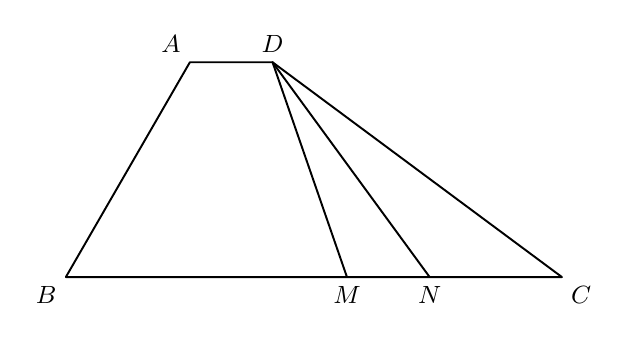
\begin{tikzpicture}[font=\small, line width=0.7pt,
  x=1.05cm, y=1.05cm, line cap=round, line join=round]
  \coordinate (B) at (0,0);
  \coordinate (C) at (6,0);
  \coordinate (A) at (1.5,2.598);
  \coordinate (D) at (2.5,2.598);
  \coordinate (M) at (3.4,0);
  \coordinate (N) at (4.4,0);
  \draw (B)--(C)--(D)--(A)--cycle;
  \draw (D)--(M);
  \draw (D)--(N);
  \node[below left,inner sep=3pt] at (B) {$B$};
  \node[below right,inner sep=3pt] at (C) {$C$};
  \node[above left,inner sep=3pt] at (A) {$A$};
  \node[above,inner sep=3pt] at (D) {$D$};
  \node[below,inner sep=3pt] at (M) {$M$};
  \node[below,inner sep=3pt] at (N) {$N$};
\end{tikzpicture}
\end{center}
\nopagebreak[4]
\Needspace{4\baselineskip}
\textbf{解析}

\textbf{先求 $\lambda$ 的值。}

\Needspace{5\baselineskip}
以 $B$ 为原点，$BC$ 所在直线为 $x$ 轴正方向建系，则
\nopagebreak[4]
\[B(0,0),\qquad C(6,0).\]
\Needspace{5\baselineskip}
由 $\angle B=60^\circ$、$AB=3$ 得
\nopagebreak[4]
\[A\left(3\cos60^\circ,\ 3\sin60^\circ\right)=\left(\frac32,\ \frac{3\sqrt3}2\right).\]

\Needspace{5\baselineskip}
由 $\overrightarrow{AD}=\lambda\overrightarrow{BC}$ 及 $\overrightarrow{BC}=(6,0)$ 得
\nopagebreak[4]
\[\overrightarrow{AD}=(6\lambda,0),\]
\Needspace{5\baselineskip}
故
\nopagebreak[4]
\[D\left(\frac32+6\lambda,\ \frac{3\sqrt3}2\right).\]

\Needspace{5\baselineskip}
又
\nopagebreak[4]
\[\overrightarrow{AB}=B-A=\left(-\frac32,\ -\frac{3\sqrt3}2\right).\]
\Needspace{5\baselineskip}
于是
\nopagebreak[4]
\[\overrightarrow{AD}\cdot\overrightarrow{AB}=6\lambda\times\left(-\frac32\right)+0=-9\lambda .\]
\Needspace{5\baselineskip}
由已知 $\overrightarrow{AD}\cdot\overrightarrow{AB}=-\dfrac32$ 得
\nopagebreak[4]
\[-9\lambda=-\frac32\ \Longrightarrow\ \lambda=\frac16 .\]
\Needspace{5\baselineskip}
此时
\nopagebreak[4]
\[D\left(\frac32+1,\ \frac{3\sqrt3}2\right)=\left(\frac52,\ \frac{3\sqrt3}2\right),\]
即 $AD=1$，与 $AD\parallel BC$、$AD=\dfrac16BC$ 相符。

\textbf{再求 $\overrightarrow{DM}\cdot\overrightarrow{DN}$ 的最小值。}

\Needspace{5\baselineskip}
$M$，$N$ 在线段 $BC$ 上且 $\left|\overrightarrow{MN}\right|=1$，按原页图示 $M$ 在 $N$ 的左侧，故可设
\nopagebreak[4]
\[M(m,0),\qquad N(m+1,0),\qquad 0\leqslant m\leqslant5 .\]
\Needspace{5\baselineskip}
由 $D\left(\dfrac52,\dfrac{3\sqrt3}2\right)$ 得
\nopagebreak[4]
\[\overrightarrow{DM}=\left(m-\frac52,\ -\frac{3\sqrt3}2\right),\qquad \overrightarrow{DN}=\left(m+1-\frac52,\ -\frac{3\sqrt3}2\right)=\left(m-\frac32,\ -\frac{3\sqrt3}2\right).\]
\Needspace{5\baselineskip}
故
\nopagebreak[4]
\[\begin{aligned}
\overrightarrow{DM}\cdot\overrightarrow{DN}
&=\left(m-\frac52\right)\left(m-\frac32\right)+\left(-\frac{3\sqrt3}2\right)^2\\
&=m^2-4m+\frac{15}4+\frac{27}4\\
&=m^2-4m+\frac{42}4\\
&=(m-2)^2+\frac{42}4-4\\
&=(m-2)^2+\frac{13}2 .
\end{aligned}\]
\Needspace{5\baselineskip}
因为 $m=2$ 落在 $[0,5]$ 内（此时 $M(2,0)$，$N(3,0)$ 都在线段 $BC$ 上），故最小值为
\nopagebreak[4]
\[\frac{13}2 .\]

填 $\dfrac16$；$\dfrac{13}2$。

\gkanswer{答案：$\dfrac16$；$\dfrac{13}2$。以 $B$ 为原点、$BC$ 为 $x$ 轴建系得 $A\left(\dfrac32,\dfrac{3\sqrt3}2\right)$，由 $\overrightarrow{AD}\cdot\overrightarrow{AB}=-9\lambda=-\dfrac32$ 得 $\lambda=\dfrac16$；再设 $M(m,0)$，则 $\overrightarrow{DM}\cdot\overrightarrow{DN}=(m-2)^2+\dfrac{13}2\geqslant\dfrac{13}2$。}

\end{answer}
\begin{answer}
\gksolhead{16}{}

\textbf{题目}：

在 $\triangle ABC$ 中，角 $A$，$B$，$C$ 所对的边分别为 $a$，$b$，$c$。已知 $a=2\sqrt2$，$b=5$，$c=\sqrt{13}$。

（1） 求角 $C$ 的大小；

（2） 求 $\sin A$ 的值；

（3） 求 $\sin\left(2A+\dfrac\pi4\right)$ 的值。

\Needspace{4\baselineskip}
\textbf{解析}

\gksubpart{（1）}

\Needspace{5\baselineskip}
由余弦定理，
\nopagebreak[4]
\[\cos C=\frac{a^2+b^2-c^2}{2ab}=\frac{(2\sqrt2)^2+5^2-(\sqrt{13})^2}{2\times2\sqrt2\times5}=\frac{8+25-13}{20\sqrt2}=\frac{20}{20\sqrt2}=\frac{\sqrt2}2 .\]
\Needspace{5\baselineskip}
又 $C\in(0,\pi)$，故
\nopagebreak[4]
\[C=\frac\pi4 .\]

\gksubpart{（2）}

\Needspace{5\baselineskip}
由正弦定理 $\dfrac a{\sin A}=\dfrac c{\sin C}$ 得
\nopagebreak[4]
\[\sin A=\frac{a\sin C}{c}=\frac{2\sqrt2\times\dfrac{\sqrt2}2}{\sqrt{13}}=\frac{2}{\sqrt{13}}=\frac{2\sqrt{13}}{13} .\]
（因 $a=2\sqrt2<5=b$，故 $A$ 为锐角，上述正弦值唯一对应一个锐角。）

\gksubpart{（3）}

\Needspace{5\baselineskip}
由（2）及 $A$ 为锐角，
\nopagebreak[4]
\[\cos A=\sqrt{1-\sin^2A}=\sqrt{1-\frac4{13}}=\sqrt{\frac9{13}}=\frac3{\sqrt{13}} .\]
\Needspace{5\baselineskip}
于是
\nopagebreak[4]
\[\sin2A=2\sin A\cos A=2\times\frac2{\sqrt{13}}\times\frac3{\sqrt{13}}=\frac{12}{13},\]
\nopagebreak[4]
\[\cos2A=\cos^2A-\sin^2A=\frac9{13}-\frac4{13}=\frac5{13} .\]
\Needspace{5\baselineskip}
故
\nopagebreak[4]
\[\begin{aligned}
\sin\left(2A+\frac\pi4\right)
&=\sin2A\cos\frac\pi4+\cos2A\sin\frac\pi4\\
&=\frac{\sqrt2}2\left(\sin2A+\cos2A\right)\\
&=\frac{\sqrt2}2\times\frac{12+5}{13}\\
&=\frac{17\sqrt2}{26} .
\end{aligned}\]

\gkanswer{答案（1）：$C=\dfrac\pi4$。由 $\cos C=\dfrac{a^2+b^2-c^2}{2ab}=\dfrac{\sqrt2}2$ 得 $C=\dfrac\pi4$。}

\gkanswer{答案（2）：$\sin A=\dfrac{2\sqrt{13}}{13}$。由正弦定理 $\sin A=\dfrac{a\sin C}{c}=\dfrac{2\sqrt2\cdot\frac{\sqrt2}2}{\sqrt{13}}=\dfrac2{\sqrt{13}}$。}

\gkanswer{答案（3）：$\sin\left(2A+\dfrac\pi4\right)=\dfrac{17\sqrt2}{26}$。由 $\cos A=\dfrac3{\sqrt{13}}$ 得 $\sin2A=\dfrac{12}{13}$、$\cos2A=\dfrac5{13}$，故原式为 $\dfrac{17}{13\sqrt2}=\dfrac{17\sqrt2}{26}$。}

\end{answer}
\begin{answer}
\gksolhead{17}{}

\textbf{题目}：

如图，在三棱柱 $ABC-A_1B_1C_1$ 中，$CC_1\perp$ 平面 $ABC$，$AC\perp BC$，$AC=BC=2$，$CC_1=3$，点 $D$，$E$ 分别在棱 $AA_1$ 和棱 $CC_1$ 上，且 $AD=1$，$CE=2$，$M$ 为棱 $A_1B_1$ 的中点。

（1） 求证：$C_1M\perp B_1D$；

（2） 求二面角 $B-B_1E-D$ 的正弦值；

（3） 求直线 $AB$ 与平面 $DB_1E$ 所成角的正弦值。
\nopagebreak[4]
\begin{center}% 2020 天津卷 第 17 题：三棱柱 ABC-A1B1C1，D 在 AA1、E 在 CC1、M 为 A1B1 中点
% 来源 PDF：普通高考/2020/2020天津.pdf 第 1 页（A3 横排），印面 1131，第 17 题题干右侧
% 几何按原页矢量数据（单位 pt，y 向下）换算为图面坐标：A(1023.5,666.2)、B(1130.9,638.1)、
%   C(1051.6,638.1)、A1(1023.5,547.1)、B1(1130.9,519.1)、C1(1051.6,519.1)；
%   即顶面 A1B1C1 由底面 ABC 竖直平移得到（侧棱 AA1、BB1、CC1 在图面上等长），
%   与 CC1 ⊥ 平面 ABC 的直棱柱一致。D 在 AA1 上且 AD:DA1 = 1:2，E 在 CC1 上且 CE:EC1 = 2:1，
%   M 为 A1B1 中点。
% 原页线型：实线 AB、AA1、BB1、A1B1、A1C1、C1B1、C1M、B1D；
%   虚线 AC、BC、CC1（被前面 ABB1A1 遮挡）、B1E、DE。
\begin{tikzpicture}[font=\small, line width=0.7pt,
  x=1.75cm, y=1.75cm, line cap=round, line join=round]
  \coordinate (A)  at (0,0);
  \coordinate (B)  at (2.68,0.70);
  \coordinate (C)  at (0.70,0.70);
  \coordinate (A1) at (0,2.98);
  \coordinate (B1) at (2.68,3.68);
  \coordinate (C1) at (0.70,3.68);
  \coordinate (D)  at (0,0.99);
  \coordinate (E)  at (0.70,2.69);
  \coordinate (M)  at ($(A1)!0.5!(B1)$);
  % 可见棱与辅助线
  \draw (A)--(B)--(B1)--(A1)--cycle;
  \draw (A1)--(C1)--(B1);
  \draw (B1)--(D);
  \draw (C1)--(M);
  % 被遮挡的棱与体内线段
  \draw[dashed] (A)--(C)--(B);
  \draw[dashed] (C)--(C1);
  \draw[dashed] (B1)--(E);
  \draw[dashed] (D)--(E);
  % 顶点标注
  \node[below left,inner sep=3pt] at (A) {$A$};
  \node[below right,inner sep=3pt] at (B) {$B$};
  \node[above right,inner sep=3pt] at (C) {$C$};
  \node[left,inner sep=3pt] at (A1) {$A_1$};
  \node[right,inner sep=3pt] at (B1) {$B_1$};
  \node[above,inner sep=2pt] at (C1) {$C_1$};
  \node[left,inner sep=3pt] at (D) {$D$};
  \node[left,inner sep=3pt] at (E) {$E$};
  \node[below,inner sep=2pt] at (M) {$M$};
\end{tikzpicture}
\end{center}
\nopagebreak[4]
\Needspace{4\baselineskip}
\textbf{解析}

\Needspace{5\baselineskip}
由 $CC_1\perp$ 平面 $ABC$ 知 $CC_1\perp CA$，$CC_1\perp CB$；又 $AC\perp BC$，故 $CA$，$CB$，$CC_1$ 两两垂直。以 $C$ 为原点，$\overrightarrow{CA}$，$\overrightarrow{CB}$，$\overrightarrow{CC_1}$ 的方向分别为 $x$，$y$，$z$ 轴正方向建系，则
\nopagebreak[4]
\[\begin{aligned}
&C(0,0,0),\quad A(2,0,0),\quad B(0,2,0),\quad C_1(0,0,3),\\
&A_1(2,0,3),\quad B_1(0,2,3).
\end{aligned}\]
\Needspace{5\baselineskip}
由 $AD=1$、$D$ 在 $AA_1$ 上得 $D(2,0,1)$；由 $CE=2$、$E$ 在 $CC_1$ 上得 $E(0,0,2)$；$M$ 为 $A_1B_1$ 的中点，故
\nopagebreak[4]
\[M\left(\frac{2+0}2,\frac{0+2}2,\frac{3+3}2\right)=(1,1,3).\]

\gksubpart{（1）}

\nopagebreak[4]
\[\overrightarrow{C_1M}=M-C_1=(1,1,0),\qquad \overrightarrow{B_1D}=D-B_1=(2,-2,-2).\]
\Needspace{5\baselineskip}
数量积
\nopagebreak[4]
\[\overrightarrow{C_1M}\cdot\overrightarrow{B_1D}=1\times2+1\times(-2)+0\times(-2)=0,\]
故 $C_1M\perp B_1D$。

\gksubpart{（2）}

\Needspace{5\baselineskip}
平面 $BB_1E$ 中三点 $B(0,2,0)$，$B_1(0,2,3)$，$E(0,0,2)$ 的 $x$ 坐标都是 $0$，故该平面即 $x=0$，其法向量可取
\nopagebreak[4]
\[\boldsymbol n_1=(1,0,0).\]

\Needspace{5\baselineskip}
平面 $DB_1E$ 中
\nopagebreak[4]
\[\overrightarrow{B_1D}=(2,-2,-2),\qquad \overrightarrow{B_1E}=E-B_1=(0,-2,-1).\]
\Needspace{5\baselineskip}
取法向量
\nopagebreak[4]
\[\boldsymbol n_2=\overrightarrow{B_1D}\times\overrightarrow{B_1E}=
\begin{vmatrix}
\boldsymbol i&\boldsymbol j&\boldsymbol k\\
2&-2&-2\\
0&-2&-1
\end{vmatrix}
=(-2,\ 2,\ -4),\]
\Needspace{5\baselineskip}
三个分量依次为 $(-2)(-1)-(-2)(-2)=-2$、$-[2\times(-1)-(-2)\times0]=2$、$2\times(-2)-(-2)\times0=-4$。把 $\boldsymbol n_2$ 乘以 $-1$ 仍为法向量，为便于计算取
\nopagebreak[4]
\[\boldsymbol n_2=(1,-1,2).\]

\Needspace{5\baselineskip}
设两平面夹角为 $\theta$，则
\nopagebreak[4]
\[\cos\theta=\frac{|\boldsymbol n_1\cdot\boldsymbol n_2|}{|\boldsymbol n_1||\boldsymbol n_2|}=\frac{|1\times1+0+0|}{1\times\sqrt{1+1+4}}=\frac1{\sqrt6} .\]
\Needspace{5\baselineskip}
故二面角的正弦值为
\nopagebreak[4]
\[\sin\theta=\sqrt{1-\frac16}=\sqrt{\frac56}=\frac{\sqrt{30}}6 .\]

\gksubpart{（3）}

\nopagebreak[4]
\[\overrightarrow{AB}=B-A=(-2,2,0),\qquad |\overrightarrow{AB}|=\sqrt{4+4}=2\sqrt2 .\]
\Needspace{5\baselineskip}
平面 $DB_1E$ 的法向量仍取 $\boldsymbol n_2=(1,-1,2)$，$|\boldsymbol n_2|=\sqrt6$。设直线 $AB$ 与平面 $DB_1E$ 所成角为 $\varphi$，则
\nopagebreak[4]
\[\sin\varphi=\frac{|\overrightarrow{AB}\cdot\boldsymbol n_2|}{|\overrightarrow{AB}||\boldsymbol n_2|}=\frac{|(-2)\times1+2\times(-1)+0\times2|}{2\sqrt2\times\sqrt6}=\frac{|-4|}{2\sqrt{12}}=\frac4{4\sqrt3}=\frac{\sqrt3}3 .\]

\gkanswer{答案（1）：证明。以 $C$ 为原点、$CA$、$CB$、$CC_1$ 为三轴建系，得 $\overrightarrow{C_1M}=(1,1,0)$、$\overrightarrow{B_1D}=(2,-2,-2)$，数量积为 $0$。}

\gkanswer{答案（2）：$\dfrac{\sqrt{30}}6$。平面 $BB_1E$ 即 $x=0$，平面 $DB_1E$ 的法向量为 $(1,-1,2)$，两法向量夹角余弦为 $\dfrac1{\sqrt6}$，故二面角正弦为 $\sqrt{1-\dfrac16}=\dfrac{\sqrt{30}}6$。}

\gkanswer{答案（3）：$\dfrac{\sqrt3}3$。$\overrightarrow{AB}=(-2,2,0)$ 与平面 $DB_1E$ 的法向量 $(1,-1,2)$ 夹角的余弦绝对值为 $\dfrac{|{-2-2}|}{2\sqrt2\cdot\sqrt6}=\dfrac{1}{\sqrt3}$，直线与平面所成角的正弦值即为此值。}

\end{answer}
\begin{answer}
\gksolhead{18}{}

\textbf{题目}：

已知椭圆 $\dfrac{x^2}{a^2}+\dfrac{y^2}{b^2}=1$（$a>b>0$）的一个顶点为 $A(0,-3)$，右焦点为 $F$，且 $|OA|=|OF|$，其中 $O$ 为原点。

（1） 求椭圆方程；

（2） 已知点 $C$ 满足 $3\overrightarrow{OC}=\overrightarrow{OF}$，点 $B$ 在椭圆上（$B$ 异于椭圆的顶点），直线 $AB$ 与以 $C$ 为圆心的圆相切于点 $P$，且 $P$ 为线段 $AB$ 的中点。求直线 $AB$ 的方程。

\Needspace{4\baselineskip}
\textbf{解析}

\gksubpart{（1）}

顶点 $A(0,-3)$ 在 $y$ 轴上，故 $b=3$（因 $a>b>0$，$y$ 轴上的顶点到原点距离为 $b$）。

\Needspace{5\baselineskip}
右焦点 $F(c,0)$，其中 $c=\sqrt{a^2-b^2}$。由 $|OA|=|OF|$ 得
\nopagebreak[4]
\[3=|OF|=c .\]
\Needspace{5\baselineskip}
于是
\nopagebreak[4]
\[a^2=b^2+c^2=9+9=18 .\]
\Needspace{5\baselineskip}
椭圆方程为
\nopagebreak[4]
\[\frac{x^2}{18}+\frac{y^2}9=1 .\]

\gksubpart{（2）}

\Needspace{5\baselineskip}
由（1）$F(3,0)$。设 $C(x_C,y_C)$，由 $3\overrightarrow{OC}=\overrightarrow{OF}$ 得
\nopagebreak[4]
\[3(x_C,y_C)=(3,0)\ \Longrightarrow\ C(1,0).\]

\Needspace{5\baselineskip}
设直线 $AB$ 的斜率为 $k$，由 $A(0,-3)$ 得
\nopagebreak[4]
\[AB:\ y=kx-3 .\]
\Needspace{5\baselineskip}
因 $B$ 在椭圆上且 $B\neq A$，设 $B(u,ku-3)$，则 $u\neq0$，且
\nopagebreak[4]
\[\frac{u^2}{18}+\frac{(ku-3)^2}9=1 .\]
\Needspace{5\baselineskip}
两边乘 $18$：
\nopagebreak[4]
\[u^2+2(ku-3)^2=18\ \Longrightarrow\ u^2+2k^2u^2-12ku+18=18,\]
\Needspace{5\baselineskip}
即
\nopagebreak[4]
\[u^2(1+2k^2)-12ku=0\ \Longrightarrow\ u\left[(1+2k^2)u-12k\right]=0 .\]
\Needspace{5\baselineskip}
由 $u\neq0$ 得
\nopagebreak[4]
\[u=\frac{12k}{1+2k^2}. \tag{1}\]

\Needspace{5\baselineskip}
$P$ 为线段 $AB$ 的中点，故
\nopagebreak[4]
\[P\left(\frac u2,\ \frac{ku-3-3}2\right)=\left(\frac u2,\ \frac{ku-6}2\right).\]
\Needspace{5\baselineskip}
圆以 $C$ 为圆心、与 $AB$ 相切于 $P$，故 $CP\perp AB$，即 $\overrightarrow{CP}\cdot(1,k)=0$：
\nopagebreak[4]
\[\left(\frac u2-1\right)\times1+\frac{ku-6}2\times k=0 .\]
\Needspace{5\baselineskip}
两边乘 $2$：
\nopagebreak[4]
\[u-2+k^2u-6k=0\ \Longrightarrow\ u(1+k^2)=2+6k\ \Longrightarrow\ u=\frac{2+6k}{1+k^2}. \tag{2}\]

\Needspace{5\baselineskip}
由（1）（2）得
\nopagebreak[4]
\[\frac{12k}{1+2k^2}=\frac{2+6k}{1+k^2},\]
\Needspace{5\baselineskip}
即
\nopagebreak[4]
\[12k(1+k^2)=(2+6k)(1+2k^2).\]
\Needspace{5\baselineskip}
展开：
\nopagebreak[4]
\[12k+12k^3=2+6k+4k^2+12k^3\ \Longrightarrow\ 4k^2-6k+2=0\ \Longrightarrow\ 2k^2-3k+1=0,\]
\Needspace{5\baselineskip}
故
\nopagebreak[4]
\[(2k-1)(k-1)=0\ \Longrightarrow\ k=\frac12\ \text{\text{或}}\ k=1 .\]

检验两解：

\begin{itemize}
\item $k=1$：由（1）$u=\dfrac{12}{3}=4$，$B(4,1)$，代入椭圆 $\dfrac{16}{18}+\dfrac19=\dfrac89+\dfrac19=1$，成立；$B$ 不是顶点。
\item $k=\dfrac12$：由（1）$u=\dfrac{6}{1+\frac12}=\dfrac{6}{\frac32}=4$，$B\left(4,\dfrac12\times4-3\right)=(4,-1)$，代入椭圆同样成立；$B$ 不是顶点。
\end{itemize}

\Needspace{5\baselineskip}
故直线 $AB$ 的方程为
\nopagebreak[4]
\[y=x-3\quad\text{\text{或}}\quad y=\frac12x-3 .\]

\gkanswer{答案（1）：$\dfrac{x^2}{18}+\dfrac{y^2}9=1$。顶点 $A(0,-3)$ 给出 $b=3$，$|OF|=|OA|=3$ 给出 $c=3$，故 $a^2=b^2+c^2=18$。}

\gkanswer{答案（2）：$y=x-3$ 或 $y=\dfrac12x-3$。设 $AB:y=kx-3$，$B(u,ku-3)$ 在椭圆上给出 $u=\dfrac{12k}{1+2k^2}$，$CP\perp AB$ 给出 $u=\dfrac{2+6k}{1+k^2}$，联立得 $(2k-1)(k-1)=0$。}

\end{answer}
\begin{answer}
\gksolhead{19}{}

\textbf{题目}：

已知 $\{a_n\}$ 为等差数列，$\{b_n\}$ 为等比数列，$a_1=b_1=1$，$a_5=5(a_4-a_3)$，$b_5=4(b_4-b_3)$。

（1） 求 $\{a_n\}$ 和 $\{b_n\}$ 的通项公式；

（2） 记 $\{a_n\}$ 的前 $n$ 项和为 $S_n$，求证：$S_nS_{n+2}<S_{n+1}^2$（$n\in\mathbf N^*$）；

\Needspace{5\baselineskip}
（3） 对任意的正整数 $n$，设
\nopagebreak[4]
\[c_n=\begin{cases}\dfrac{(3a_n-2)b_n}{a_na_{n+2}},&n\text{ \text{为奇数}},\\[2ex]\dfrac{a_{n-1}}{b_{n+1}},&n\text{ \text{为偶数}}.\end{cases}\]
求数列 $\{c_n\}$ 的前 $2n$ 项和。

\Needspace{4\baselineskip}
\textbf{解析}

\gksubpart{（1）}

\Needspace{5\baselineskip}
设 $\{a_n\}$ 的公差为 $d$，则 $a_4-a_3=d$，$a_5=a_1+4d=1+4d$。由 $a_5=5(a_4-a_3)$ 得
\nopagebreak[4]
\[1+4d=5d\ \Longrightarrow\ d=1,\]
\Needspace{5\baselineskip}
故
\nopagebreak[4]
\[a_n=1+(n-1)\times1=n .\]

\Needspace{5\baselineskip}
设 $\{b_n\}$ 的公比为 $q$（$b_n=b_1q^{n-1}=q^{n-1}$，故 $q\neq0$）。由 $b_5=4(b_4-b_3)$ 得
\nopagebreak[4]
\[q^4=4\left(q^3-q^2\right)=4q^2(q-1) .\]
\Needspace{5\baselineskip}
两边除以 $q^2>0$：
\nopagebreak[4]
\[q^2=4(q-1)\ \Longrightarrow\ q^2-4q+4=0\ \Longrightarrow\ (q-2)^2=0\ \Longrightarrow\ q=2 .\]
\Needspace{5\baselineskip}
故
\nopagebreak[4]
\[b_n=2^{n-1} .\]

\gksubpart{（2）}

\Needspace{5\baselineskip}
由（1）得
\nopagebreak[4]
\[S_n=\frac{n(a_1+a_n)}2=\frac{n(1+n)}2=\frac{n(n+1)}2 .\]
\Needspace{5\baselineskip}
于是
\nopagebreak[4]
\[S_nS_{n+2}=\frac{n(n+1)}2\cdot\frac{(n+2)(n+3)}2,\qquad S_{n+1}^2=\left[\frac{(n+1)(n+2)}2\right]^2 .\]
\Needspace{5\baselineskip}
两者都是正数，作商比较：约去公因子 $\dfrac{(n+1)(n+2)}4$，得
\nopagebreak[4]
\[\frac{S_nS_{n+2}}{S_{n+1}^2}=\frac{n(n+3)}{(n+1)(n+2)} .\]
\Needspace{5\baselineskip}
而
\nopagebreak[4]
\[(n+1)(n+2)-n(n+3)=\left(n^2+3n+2\right)-\left(n^2+3n\right)=2>0,\]
\Needspace{5\baselineskip}
故
\nopagebreak[4]
\[\frac{n(n+3)}{(n+1)(n+2)}<1\ \Longrightarrow\ S_nS_{n+2}<S_{n+1}^2 .\]
对一切 $n\in\mathbf N^*$ 成立。

\gksubpart{（3）}

由（1）$a_n=n$，$b_n=2^{n-1}$。

\Needspace{5\baselineskip}
\textbf{奇数项。} 设 $n=2j-1$（$j=1,2,\cdots$），则
\nopagebreak[4]
\[c_{2j-1}=\frac{(3a_{2j-1}-2)b_{2j-1}}{a_{2j-1}a_{2j+1}}=\frac{(3(2j-1)-2)\cdot2^{2j-2}}{(2j-1)(2j+1)}=\frac{(6j-5)4^{j-1}}{(2j-1)(2j+1)} .\]
\Needspace{5\baselineskip}
把 $\dfrac{6j-5}{(2j-1)(2j+1)}$ 拆成部分分式：设
\nopagebreak[4]
\[\frac{6j-5}{(2j-1)(2j+1)}=\frac{A}{2j-1}+\frac{B}{2j+1},\]
\Needspace{5\baselineskip}
则 $A(2j+1)+B(2j-1)=6j-5$，比较系数得 $2A+2B=6$，$A-B=-5$，解得 $A=-1$，$B=4$。故
\nopagebreak[4]
\[\frac{6j-5}{(2j-1)(2j+1)}=-\frac1{2j-1}+\frac4{2j+1},\]
\Needspace{5\baselineskip}
乘以 $4^{j-1}$：
\nopagebreak[4]
\[c_{2j-1}=-\frac{4^{j-1}}{2j-1}+\frac{4^{j}}{2j+1} .\]
\Needspace{5\baselineskip}
这是裂项形式，求和时相邻项相消：
\nopagebreak[4]
\[\sum_{j=1}^{n}c_{2j-1}=\left(-\frac{4^0}{1}+\frac{4^1}{3}\right)+\left(-\frac{4^1}{3}+\frac{4^2}{5}\right)+\cdots+\left(-\frac{4^{n-1}}{2n-1}+\frac{4^n}{2n+1}\right)=\frac{4^n}{2n+1}-1 .\]

\Needspace{5\baselineskip}
\textbf{偶数项。} 设 $n=2j$，则
\nopagebreak[4]
\[c_{2j}=\frac{a_{2j-1}}{b_{2j+1}}=\frac{2j-1}{2^{2j}}=\frac{2j-1}{4^j} .\]
\Needspace{5\baselineskip}
记 $x=\dfrac14$，则
\nopagebreak[4]
\[\sum_{j=1}^n c_{2j}=\sum_{j=1}^n(2j-1)x^j=2\sum_{j=1}^n jx^j-\sum_{j=1}^n x^j .\]
\Needspace{5\baselineskip}
用公式 $\sum\limits_{j=1}^n jx^j=\dfrac{x\left[1-(n+1)x^n+nx^{n+1}\right]}{(1-x)^2}$ 与 $\sum\limits_{j=1}^n x^j=\dfrac{x(1-x^n)}{1-x}$，代入 $x=\dfrac14$（此时 $1-x=\dfrac34$，$(1-x)^2=\dfrac9{16}$）：
\nopagebreak[4]
\[\sum_{j=1}^n jx^j=\frac{\frac14\left[1-\frac{n+1}{4^n}+\frac n{4^{n+1}}\right]}{\frac9{16}}=\frac49\left[1-\frac{n+1}{4^n}+\frac n{4^{n+1}}\right],\]
\nopagebreak[4]
\[\sum_{j=1}^n x^j=\frac{\frac14\left(1-\frac1{4^n}\right)}{\frac34}=\frac13\left(1-\frac1{4^n}\right).\]
\Needspace{5\baselineskip}
故
\nopagebreak[4]
\[\begin{aligned}
\sum_{j=1}^n c_{2j}
&=2\times\frac49\left[1-\frac{n+1}{4^n}+\frac n{4^{n+1}}\right]-\frac13\left(1-\frac1{4^n}\right)\\
&=\frac89-\frac13-\frac{8(n+1)}{9\cdot4^n}+\frac{8n}{9\cdot4^{n+1}}+\frac1{3\cdot4^n}\\
&=\frac59+\frac1{4^n}\left[-\frac{8(n+1)}9+\frac{2n}9+\frac13\right]\\
&=\frac59+\frac1{4^n}\cdot\frac{-8n-8+2n+3}{9}\\
&=\frac59-\frac{6n+5}{9\cdot4^n} .
\end{aligned}\]

\Needspace{5\baselineskip}
\textbf{合计。} $\{c_n\}$ 的前 $2n$ 项和为
\nopagebreak[4]
\[\begin{aligned}
T_n&=\sum_{j=1}^n c_{2j-1}+\sum_{j=1}^n c_{2j}\\
&=\left(\frac{4^n}{2n+1}-1\right)+\left(\frac59-\frac{6n+5}{9\cdot4^n}\right)\\
&=\frac{4^n}{2n+1}-\frac{6n+5}{9\cdot4^n}-\frac49 .
\end{aligned}\]

数值复核：$n=1$ 时 $T_1=c_1+c_2=\dfrac13+\dfrac14=\dfrac7{12}$，而公式给出 $\dfrac43-\dfrac{11}{36}-\dfrac49=\dfrac{48-11-16}{36}=\dfrac{21}{36}=\dfrac7{12}$，相符；$n=2$ 时公式给出 $\dfrac{16}5-\dfrac{17}{144}-\dfrac49=\dfrac{211}{80}$，逐项相加 $c_1+c_2+c_3+c_4=\dfrac13+\dfrac14+\dfrac{28}{15}+\dfrac3{16}=\dfrac{211}{80}$，亦相符。

\gkanswer{答案（1）：$a_n=n$，$b_n=2^{n-1}$。由 $a_5=5(a_4-a_3)$ 得公差 $d=1$；由 $b_5=4(b_4-b_3)$ 得 $q^2=4(q-1)$，即 $(q-2)^2=0$，$q=2$。}

\gkanswer{答案（2）：证明。$S_n=\dfrac{n(n+1)}2$，不等式两边约去 $\dfrac{(n+1)(n+2)}4$ 后化为 $n(n+3)<(n+1)(n+2)$，即 $0<2$。}

\gkanswer{答案（3）：$\dfrac{4^n}{2n+1}-\dfrac{6n+5}{9\cdot4^n}-\dfrac49$。奇数项满足 $\dfrac{(6j-5)4^{j-1}}{(2j-1)(2j+1)}=\dfrac{4^j}{2j+1}-\dfrac{4^{j-1}}{2j-1}$ 可裂项，偶数项为等比与等差之积，分组求和。}

\end{answer}
\begin{answer}
\gksolhead{20}{}

\textbf{题目}：

已知函数 $f(x)=x^3+k\ln x$（$k\in\mathbf R$），$f'(x)$ 为 $f(x)$ 的导函数。

（1） 当 $k=6$ 时，

① 求曲线 $y=f(x)$ 在点 $(1,f(1))$ 处的切线方程；

② 求函数 $g(x)=f(x)-f'(x)+\dfrac9x$ 的单调区间和极值；

\Needspace{5\baselineskip}
（2） 当 $k\geqslant-3$ 时，求证：对任意的 $x_1$，$x_2\in[1,+\infty)$，且 $x_1>x_2$，有
\nopagebreak[4]
\[\frac{f'(x_1)+f'(x_2)}{2}>\frac{f(x_1)-f(x_2)}{x_1-x_2}.\]

\Needspace{4\baselineskip}
\textbf{解析}

\Needspace{5\baselineskip}
$f(x)=x^3+k\ln x$ 的定义域为 $(0,+\infty)$，且
\nopagebreak[4]
\[f'(x)=3x^2+\frac kx .\]

\gksubpart{（1）}

此时 $k=6$，$f(x)=x^3+6\ln x$，$f'(x)=3x^2+\dfrac6x$。

\Needspace{5\baselineskip}
\textbf{① 切线方程。}
\nopagebreak[4]
\[f(1)=1+6\ln1=1,\qquad f'(1)=3+6=9 .\]
\Needspace{5\baselineskip}
故曲线在点 $(1,1)$ 处的切线为
\nopagebreak[4]
\[y-1=9(x-1)\ \Longrightarrow\ y=9x-8 .\]

\Needspace{5\baselineskip}
\textbf{② $g(x)$ 的单调区间与极值。}

\nopagebreak[4]
\[\begin{aligned}
g(x)&=f(x)-f'(x)+\frac9x\\
&=\left(x^3+6\ln x\right)-\left(3x^2+\frac6x\right)+\frac9x\\
&=x^3-3x^2+6\ln x+\frac3x .
\end{aligned}\]
\Needspace{5\baselineskip}
求导：
\nopagebreak[4]
\[\begin{aligned}
g'(x)&=3x^2-6x+\frac6x-\frac3{x^2}\\
&=\frac{3x^4-6x^3+6x-3}{x^2}\\
&=\frac{3\left(x^4-2x^3+2x-1\right)}{x^2} .
\end{aligned}\]
\Needspace{5\baselineskip}
分解 $x^4-2x^3+2x-1$：$x=1$ 是其根，用综合除法
\nopagebreak[4]
\[x^4-2x^3+0x^2+2x-1=(x-1)\left(x^3-x^2-x+1\right),\]
\Needspace{5\baselineskip}
而 $x^3-x^2-x+1=x^2(x-1)-(x-1)=(x-1)\left(x^2-1\right)=(x-1)^2(x+1)$。故
\nopagebreak[4]
\[x^4-2x^3+2x-1=(x-1)^3(x+1),\]
\Needspace{5\baselineskip}
即
\nopagebreak[4]
\[g'(x)=\frac{3(x-1)^3(x+1)}{x^2} .\]
在定义域 $x>0$ 上，$x^2>0$，$x+1>0$，故 $g'(x)$ 的符号只由 $(x-1)^3$ 决定：

\begin{itemize}
\item $0<x<1$ 时 $g'(x)<0$，$g$ 单调递减；
\item $x>1$ 时 $g'(x)>0$，$g$ 单调递增。
\end{itemize}

\Needspace{5\baselineskip}
所以 $g$ 的单调递减区间为 $(0,1)$，单调递增区间为 $(1,+\infty)$，在 $x=1$ 处取极小值
\nopagebreak[4]
\[g(1)=1-3+0+3=1,\]
无极大值。

\gksubpart{（2）}

\Needspace{5\baselineskip}
设 $x_1>x_2\geqslant1$。要证
\nopagebreak[4]
\[\frac{f'(x_1)+f'(x_2)}2>\frac{f(x_1)-f(x_2)}{x_1-x_2},\]
\Needspace{5\baselineskip}
等价于（两边乘 $x_1-x_2>0$）
\nopagebreak[4]
\[f(x_1)-f(x_2)-\frac{x_1-x_2}2\left[f'(x_1)+f'(x_2)\right]<0 .\]

\Needspace{5\baselineskip}
固定 $x_2$，对 $x\geqslant x_2$ 定义
\nopagebreak[4]
\[F(x)=f(x)-f(x_2)-\frac{x-x_2}2\left[f'(x)+f'(x_2)\right].\]
则 $F(x_2)=0$，只需证 $x>x_2$ 时 $F(x)<0$。

\Needspace{5\baselineskip}
求导：
\nopagebreak[4]
\[\begin{aligned}
F'(x)&=f'(x)-\frac12\left[f'(x)+f'(x_2)\right]-\frac{x-x_2}2f''(x)\\
&=\frac{f'(x)-f'(x_2)}2-\frac{x-x_2}2f''(x).
\end{aligned}\]
\Needspace{5\baselineskip}
由 $f'(x)=3x^2+\dfrac kx$ 得 $f''(x)=6x-\dfrac k{x^2}$，于是
\nopagebreak[4]
\[\begin{aligned}
2F'(x)&=3\left(x^2-x_2^2\right)+k\left(\frac1x-\frac1{x_2}\right)-(x-x_2)\left(6x-\frac k{x^2}\right)\\
&=(x-x_2)\left[3(x+x_2)-\frac{k}{xx_2}-6x+\frac k{x^2}\right]\\
&=(x-x_2)\left[-3(x-x_2)+k\left(\frac1{x^2}-\frac1{xx_2}\right)\right].
\end{aligned}\]
\Needspace{5\baselineskip}
其中
\nopagebreak[4]
\[\frac1{x^2}-\frac1{xx_2}=\frac{x_2-x}{x^2x_2}=-\frac{x-x_2}{x^2x_2},\]
\Needspace{5\baselineskip}
故
\nopagebreak[4]
\[2F'(x)=-(x-x_2)^2\left(3+\frac{k}{x^2x_2}\right),\]
\Needspace{5\baselineskip}
即
\nopagebreak[4]
\[F'(x)=-\frac{(x-x_2)^2}2\left(3+\frac{k}{x^2x_2}\right).\]

因 $x\geqslant x_2\geqslant1$，有 $x^2x_2\geqslant1$。

\begin{itemize}
\item 若 $k\geqslant0$，则 $\dfrac{k}{x^2x_2}\geqslant0$，括号内 $>0$；
\item 若 $-3\leqslant k<0$，则 $\dfrac{k}{x^2x_2}\geqslant\dfrac{k}{1}=k\geqslant-3$，括号内 $\geqslant0$。
\end{itemize}

总之 $3+\dfrac{k}{x^2x_2}\geqslant0$，故 $F'(x)\leqslant0$，$F$ 在 $[x_2,+\infty)$ 上单调不增。

\Needspace{5\baselineskip}
注意到 $F'(x)$ 的零点只能来自因子 $(x-x_2)^2$，即只有 $x=x_2$ 处 $F'=0$；在 $(x_2,+\infty)$ 上恒有 $F'(x)<0$，故 $F$ 在 $[x_2,+\infty)$ 上严格递减。于是对 $x_1>x_2$ 有
\nopagebreak[4]
\[F(x_1)<F(x_2)=0,\]
即原不等式严格成立。

\Needspace{5\baselineskip}
综上，当 $k\geqslant-3$ 时，对任意 $x_1>x_2\geqslant1$ 都有
\nopagebreak[4]
\[\frac{f'(x_1)+f'(x_2)}2>\frac{f(x_1)-f(x_2)}{x_1-x_2}.\]

\Needspace{5\baselineskip}
数值复核：取 $k=-3$，$x_2=1$，$x_1=1.5$，则
\nopagebreak[4]
\[\frac{f'(x_1)+f'(x_2)}2=\frac{(3\times2.25-2)+(3-3)}2=\frac{4.75}2=2.375,\]
\nopagebreak[4]
\[\frac{f(x_1)-f(x_2)}{x_1-x_2}=\frac{(3.375-3\ln1.5)-1}{0.5}\approx\frac{3.375-1.2164-1}{0.5}=2.317,\]
两者之差为 $0.058>0$，与结论一致；同法在 $k=-3$ 与 $x_1,x_2\geqslant1$ 的网格上扫描，差的最小值为 $0$（仅在 $x_1\to x_2$ 的极限处取到），不出现负值。

\gkanswer{答案（1）：① $y=9x-8$；② 单调递减区间 $(0,1)$，单调递增区间 $(1,+\infty)$，极小值 $g(1)=1$，无极大值。$f(1)=1$、$f'(1)=9$ 给出切线；$g'(x)=\dfrac{3(x-1)^3(x+1)}{x^2}$ 定号即得单调性与极值。}

\gkanswer{答案（2）：证明。令 $F(x)=f(x)-f(x_2)-\dfrac{x-x_2}2\left[f'(x)+f'(x_2)\right]$，则 $F(x_2)=0$ 且 $F'(x)=-\dfrac{(x-x_2)^2}2\left(3+\dfrac{k}{x^2x_2}\right)$；由 $x\geqslant x_2\geqslant1$、$k\geqslant-3$ 得括号内非负，故 $F$ 严格递减，$F(x_1)<0$ 即所证。}

\end{answer}